
\chapter{II. Courants, sensibilités, figures de l’islam de France (ii)}

\mn{LUNDI 6 DECEMBRE 2021 (3e
cours) }

%------------------------------------------------------------------------------------------------

\section{« Islams consulaires » : les pays d’origine dans l’équation de l’islam de
France}

\mn{Issu du rapport montaigne}
\paragraph{Une organisation par le haut}

L'islam en France est fragmenté, parcellaire et composite. On y trouve
des acteurs historiques, présents dès l'établissement de l'islam en
France : ce sont les États d'origine des Français de confession
musulmane, à qui l'État a délégué, par commodité juridique et pratique,
la gestion de l'islam et l'encadrement des musulmans (2.1). D'autres
acteurs ont émergé progressivement, au fur et à mesure de la
structuration du culte musulman, et continuent aujourd'hui de jouer un
rôle important dans les dynamiques qui traversent l'islam français. Ce
sont les Frères Musulmans, organisés en une Union des Organisations
islamiques de France (UOIF),qui promeuvent une nouvelle forme de
religiosité en investissant le champ politique (2.2), d'une part ; ce
sont les salafistes qui, sous l'effet conjoint de l'affaissement du
militantisme politique et de la néo-islamisation des jeunes, sont
apparus comme un acteur de plus en plus important, même sans structure
centralisée (2.4), d'autre part. Enfin, il convient d'évoquer la
tentative, imparfaite, menée par l'État afin de mettre en place des
structures d'organisation d'un islam français (2.3). Cette dernière
question est mise en avant par le Gouvernement depuis plusieurs semaines
et ce rapport espère y avoir contribué.



\paragraph{L'islam Consulaire}


Dans l'ensemble de l'Europe, la gestion de l'islam a été déléguée à des
États étrangers pendant plusieurs décennies. Ces États, dont sont
souvent originaires les musulmans d'Europe, ont exercé un puissant
contrôle sur l'islam européen, dès l'arrivée massive des premiers
immigrés au tournant des années 1950. Les États européens ont longtemps
bénéficié de cette situation qui leur épargnait de s'immiscer dans la
gestion et la régulation de l'islam, en partie car, jusqu'au milieu des
années 1970, l'installation des travailleurs immigrés était perçue comme
provisoire. Aussi, pendant plusieurs décennies, les intérêts des États
d'accueil et des États d'origine étaient-ils relativement alignés. La
présence de travailleurs immigrés musulmans était perçue comme
temporaire et l'islam était, par conséquent, perçu comme une réalité
exogène ; ainsi les pays d'accueil ont- ils évité de s'enferrer dans
l'épineuse question du statut de l'islam dans les sociétés européennes.
Lorsque la présence de ces immigrés musulmans s'est avérée durable, les
États ont adopté une politique pragmatique : à défaut de pouvoir
endiguer l'influence 
étrangère, ils ont favorisé le recrutement d'imams par les réseaux
consulaires, pensant ainsi éviter les dérives fondamentalistes et
islamistes. Les États étrangers trouvaient par ailleurs un intérêt
certain dans la gestion à distance de l'islam en Europe, car il
s'agissait d'un moyen de maintenir à la fois un contrôle et des liens
avec cette population émigrée, mais aussi d'éviter que lors de leurs
visites « au bled » les immigrés ne soient les vecteurs d'une
contamination islamiste. Ainsi, jusqu'à la fin des années 1970, les
Européens ont développé des politiques d'intégration conçues dans
l'optique d'un retour futur qui coïncidait plutôt bien avec les
intentions religieuses et culturelles des trois principaux pays de
départ -- l'Algérie, le Maroc et la Turquie -- ainsi qu'avec les
aspirations à l'hégémonie religieuse des hauts responsables d'Arabie
Saoudite.

Si, durant la période qui s'étend de la fin des années 1950 à
aujourd'hui, les États d'origine ont soutenu -- sinon accru -- leurs
efforts afin de maintenir leur contrôle sur les populations émigrées, on
peut toutefois distinguer deux formes d'islam consulaire : celui des
États émetteurs de population et celui des États émetteurs d'idéologie.


\begin{enumerate}

\item
  
  \textbf{Le modèle d'islam consulaire développé par les États émetteurs
  de population, au premier rang desquels l'Algérie, le Maroc et la
  Turquie, s'insère dans le modèle plus large du contrôle des
  populations émigrées.} Le discours développé par chacun de ces États
  s'effectue dans un double objectif : prévenir une contamination
  idéologique et fondamentaliste des populations émigrées, qui
  pourraient être susceptibles de la diffuser dans l'État d'origine, et
  maintenir des liens avec une population diasporique, qui contribue
  largement au développement économique du pays grâce aux remises
  migratoires.
  
\item
  
  \textbf{L'autre modèle d'islam consulaire est celui mis en œuvre par
  les États non émetteurs de population, à l'instar de l'Arabie Saoudite
  ou du Qatar, qui cherchent à diffuser à l'échelle mondiale une
  idéologie islamique.} Les musulmans d'Europe constituent pour eux une
  cible d'importance. C'est tout un réseau d'associations islamiques qui
  est alors développé afin d'embrasser le plus grand nombre de musulmans
  européens. Cette politique religieuse diplomatique s'inscrit plus
  largement dans une politique de soft power et d'influence.
  
\end{enumerate}
 
  \subsection{Les pays étrangers émetteurs de
    population} 


L'islam consulaire, mis en œuvre par les États émetteurs de population,
connaît trois phases principales dans son développement :


\begin{itemize}
\item
  la première période, que l'on peut dater des années 1950 à la fin des
  années 1970, correspond à la mise en place de structures islamiques à
  destination d'une population de travailleurs immigrés dont la présence
  en France est conçue comme temporaire. C'est \textbf{« l'islam des
  foyers »} ;
\item
  la seconde période, qui court de la fin des années 1970 au tournant
  des années 2000, correspond à une phase d'enracinement de la
  population musulmane en France et se caractérise par la mise en place
  des premières infrastructures religieuses grâce au soutien financier
  des États d'origine. C'est \textbf{« l'islam des quartiers »} ;
\item
  la troisième période, amorcée durant les années 1990 et qui perdure de
  nos jours, est marquée par une crise relative de l'islam consulaire :
  l'arrivée d'une nouvelle génération de musulmans, née ou socialisée en
  France et qui ne se reconnaît plus dans cet islam étranger, provoque
  un recul relatif des réseaux consulaires, qui demeurent malgré tout
  des interlocuteurs privilégiés des pouvoirs publics. C'est
\end{itemize}


\paragraph{« l'islam des institutions »}.


\subparagraph{« L'islam des foyers »}


Entre 1955 et 1974, environ 711 000 Algériens, 260 000 Marocains et 140
000 Tunisiens se sont installés en France33. Cette population
majoritairement masculine et ouvrière a participé à la reconstruction de
la France de l'après-guerre et à son développement durant les Trente
Glorieuses34. À partir des années 1970, sous l'effet du ralentissement
économique et du développement de politiques publiques orientées vers le
retour au pays de ces travailleurs immigrés, la puissance publique a
encouragé la création de salles de prières et l'implication des États
d'origine dans la prise en charge du culte : 
\begin{quote}
    La pratique
religieuse n'est jamais appréhendée comme une fin en soi, mais plutôt
comme un moyen. Aider au maintien de la religiosité des migrants vise
surtout à s'assurer que leur sentiment d'appartenance nationale reste
suffisamment vivace pour empêcher une installation pérenne sur le
territoire français. \sn{Solenne Jouanneau, \textit{Les imams en France. Une autorité religieuse sous contrôle}, Paris, Éditions Agone, coll. « L’ordre des choses », 2013, p. 51.}
\end{quote}

Des salles de prières ont ainsi été
aménagées dans les foyers de travailleurs comme dans les entreprises qui
recouraient à cette main-d'œuvre.


\subparagraph{« L'islam des quartiers »}

Le premier choc pétrolier de 1973 a entraîné la fin de l'immigration de
masse et mis fin aux discours politiques qui prévoyaient le retour à
terme des populations immigrées : l'échec du projet Stoléru de 1976,
prévoyant une aide au retour, et la mise en place du regroupement
familial, en 1978, signent la fin d'une conception relativement
illusoire de la politique migratoire. L'installation durable de ces
populations immigrées, majoritairement musulmanes, fait naître le besoin
pour la puissance publique d'avoir un interlocuteur avec lequel définir
et gérer les besoins religieux. Compte tenu de la faiblesse -- voire de
l'inexistence -- d'organisations musulmanes locales, mais aussi des
entraves juridiques qui se présentaient aux pouvoirs publics, notamment
en France du fait de la séparation des Églises et de l'État, la gestion
des salles de prière, des imams, des sacrifices rituels et du pèlerinage
à la Mecque fut alors déléguée aux pays d'origine.

Aussi cette période d'enracinement de l'islam en France est-elle marquée
par une progressive autonomisation des lieux de culte vis-à-vis des
principales structures d'encadrement de la main-d'œuvre immigrée dans
les usines et les foyers. Les lieux de culte se développent à proximité
des lieux de résidence, dans les quartiers. À partir de 1981, sous
l'effet de la libéralisation du droit d'association pour les étrangers
résidant sur le territoire (loi du 9 octobre 1981), le culte s'est
structuré autour d'associations locales et ces salles autonomes se sont
imposées comme la norme organisationnelle du culte musulman.

La délégation de l'islam aux pays d'origine s'explique également par la
crainte des États européens de voir l'islamisme se propager. L'année
1979, marquée par la révolution iranienne, la prise de la Grande Mosquée
de la Mecque et l'invasion soviétique de l'Afghanistan, a fait émerger
le spectre de l'islamisme. Le développement de l'islam consulaire dans
le paysage national européen offrait ainsi une apparente garantie de
sécurité. Dans le contexte de la Guerre froide, marqué par la résurgence
de l'islamisme, l'Algérie, le Maroc et la Turquie semblaient pouvoir
constituer un front commun qui, s'il n'était pas vraiment pro-occidental
(l'Algérie étant à l'époque un non-aligné sympathisant de l'URSS), était
au moins anti-terroriste.

\subparagraph{L'exemple des « imams-ELCO »}


Le cas des « imams-ELCO » constitue sans doute en France la
manifestation la plus visible de la coopération entre l'État et l'islam
consulaire. Créés en 1975 et gérés par l'Éducation nationale, les
programmes ELCO (Enseignement des langues et cultures d'origine)
permettent aux enfants d'origine étrangère d'apprendre la langue de leur
pays d'origine. Les États d'origine participant au programme choisissent
et salarient les enseignants, qui sont des fonctionnaires détachés,
déterminent le contenu de ces enseignements, tandis que le ministère des
Affaires étrangères octroie des visas de séjour. Ces enseignants
détachés des pays d'origine pour une durée de quatre ans sont très
majoritairement des responsables religieux, les imams ayant un statut de
fonction- naire en Algérie et en Turquie. Les « imams-ELCO » constituent
une fiction juridique qui permet à l'État d'externaliser la gestion du
culte tout en assurant un encadrement administratif. On estime qu'entre
1984 et 1992 ce sont environ 64 000 élèves d'ori- gines algérienne,
marocaine, tunisienne et turque qui ont suivi ces enseignements.

À partir de la fin des années 1980, les pouvoirs publics renforcent le
contrôle des programmes ELCO car plusieurs dérives islamistes ont été
constatées.

\subparagraph{1975-1997 : la gestion du culte grâce à une fiction juridique}
\label{par:IslamConsulaireAlgérie}
Les fonctionnaires détachés par le gouvernement algérien sont très
majoritairement des imams. Depuis 1969, ceux-ci ont le statut de
fonctionnaire et dépendent du ministère des Habous et des affaires
islamiques, qui gère à la fois les affaires religieuses et les
propriétés foncières du culte. Depuis 1981, ils sont obligatoirement
titulaires d'un diplôme d'État. Le dispositif des ELCO \emph{« permet de
tirer parti de la fonctionnarisation de l'imamat en Algérie, les
autorités algériennes venant ici suppléer l'absence d'une institution
ecclésiale islamique française et centralisée capable de définir
l'identité des clercs musulmans légitimes et d'entretenir avec ces
derniers des relations d'ordre hiérarchique ».} La gestion de ces
imams-fonctionnaires détachés en France, auparavant assurée par les
autorités consulaires algériennes, a été progressivement déléguée à la
Grande Mosquée de Paris : le ministère des Habous sélectionnait les
imams et la Grande Mosquée se chargeait de les accueillir et de les
affecter dans les différentes mosquées affiliées.
 

C'est un autre « dispositif d'externalisation diplomatique » qui est
utilisé pour les imams-fonctionnaires turcs. Les imams turcs présents en
France le sont officiellement en tant qu'assistants sociaux rémunérés
par le gouvernement turc. Leur encadrement est beaucoup plus centralisé
que celui des imams algériens. Il s'articule autour de deux entités : le
DITIB \emph{(Diyanet Işleri Türk-Islam Birliği)}, ou l'Union des
Affaires culturelles turco-islamiques, chargée de soutenir la communauté
turque, notamment en Europe, pour les questions relatives à la religion
; et le Diyanet, qui préside les affaires religieuses au sein du
gouvernement turc. Dans chaque consulat turc un représentant du DITIB\sn{ Créée dans les années 80, la DITIB (Union des Affaires Culturelles
Turco-Islamiques -- en turc \emph{« Diyanet Işleri Türk- Islam Birliği
»)} est chargée de soutenir la communauté turque notamment celle
d'Europe pour les questions relatives à la religion, d'envoyer des imams
et des enseignants de religion de Turquie, ainsi que l'aide à la
construction des mosquées et des centres culturels en Europe.}
est ainsi chargé d'inspecter les mosquées turques affiliées, tandis que
chaque imam détaché reçoit « un bulletin du Diyanet\sn{Diyanet : présidence des Affaires Religieuses au sein du gouvernement
turc. Directement rattaché au cabinet du Premier Ministre, le Diyanet a
pour mission : de s'occuper des activités liées aux croyances de la
religion de l'Islam ; d'éclairer la société sur la religion : le culte
et la morale de l'Islam ; de gérer les lieux de culte.}» qui contient
notamment les prêches du vendredi préparés par le pouvoir central turc.
Le contrôle des imams et leur lien avec le pays d'origine y est donc
beaucoup plus fort.




\subparagraph{1997-2002 : La remise en cause du dispositif des « imams-ELCO »}

Alors ministre de l'Intérieur, Jean-Pierre Chevènement a procédé à la
révision du dispositif des imams-ELCO, qui sera poursuivie par ses
successeurs. La révision du dispositif s'imposait, car des comportements
problématiques entravaient son fonctionnement.

Comme ces imams étaient étroitement liés au gouvernement de leur pays
d'origine du fait de leur statut de fonctionnaire, ils servaient de
relais politiques aux autorités consulaires et faisaient montre d'une
trop forte dépendance au contexte politique du pays d'origine.

En outre, ces imams étaient faiblement intégrés à la société française.
Leur détachement provisoire ne les incitait guère à faire de véritables
efforts d'intégration : peu maîtrisaient le français, car le prêche
devait être obligatoirement délivré dans la langue de leur pays
d'origine (une dynamique accentuée par la politique d'arabisation de
l'État algérien). De plus, étant donné qu'un détachement à l'étranger
contribuait à dynamiser une carrière pour les plus jeunes ou à la
couronner pour les plus âgés, ces imams étaient beaucoup plus attachés à
satisfaire leur hiérarchie qu'à promouvoir un islam français.

Enfin, l'impossibilité de généraliser le dispositif à toutes les
nationalités constituait une autre source de dysfonctionnement du
dispositif, puisque tous les clercs musulmans ne sont pas soumis à un
statut de fonctionnaire dans leur pays d'origine. Ils ne le sont pas au
Maroc par exemple. C'est donc une faiblesse inhérente au dispositif qui
« dans sa forme même, est extrêmement dépendant de la façon dont le
culte musulman s'est structuré dans les pays d'émigration ».

Aussi Jean Pierre Chevènement a-t-il maintenu la logique
d'externalisation du contrôle des imams étrangers \emph{via} des réseaux
consulaires mais en a renouvelé la forme. Il s'agissait de mettre fin à
la fiction juridique des imams-ELCO, de limiter la responsabilité de
l'État et d'officialiser pour la première fois le recours de la France à
des imams étrangers. Ainsi, pour les imams algériens entrés en France
avant la réforme, un examen au cas par cas avant la délivrance d'une
carte de séjour visiteur (un an renouvelable) a été effectué. Pour les
nouveaux imams, l'État n'intervient plus directement puisque le
détachement des imams résulte de la signature d'un protocole officiel
entre le gouvernement algérien et la Grande Mosquée de Paris.

La mise en place de l'islam consulaire est le produit de la combinaison
d'un « état de fait » et d'une politique publique se voulant pragmatique.
Initialement, les infrastructures cultuelles musulmanes étaient très peu
nombreuses et encore embryonnaires : les fidèles disposaient rarement de
lieux de culte adaptés (c'est l'époque de « l'islam des caves ») et la
grande majorité des associations musulmanes ne pouvaient assumer la
charge financière du traitement des imams. Les États étrangers prirent
\emph{de facto} en charge la gestion et le fonctionnement du culte. Ce
n'est que dans un second temps, notamment à partir des années 1990, que
l'État a tenté d'encadrer davantage l'islam consulaire. Ainsi, Raoul
Weexsteen, le conseiller islam de Pierre Joxe puis de Charles Pasqua, a
promu une politique pragmatique : il a favorisé le recrutement des imams
par les réseaux consulaires afin d'éviter les dérives fondamentalistes
et islamistes, à défaut de pouvoir éviter l'influence étrangère. Le
raisonnement tenu était alors qu'un imam accrédité par son État
d'origine, notamment algérien, présentait des qualités de modération, à
une époque où l'État algérien luttait contre les groupes islamiques
armés (le GIA) et que le wahhabisme commençait à gangréner le tissu
musulman français.

Alors que la puissance publique tente de structurer l'islam en France,
d'abord en réformant les programmes des ELCO, puis en mettant en place
un Conseil consultatif musulman s'appuyant sur les réseaux consulaires,
et, enfin, lorsque Charles Pasqua, en tentant d'organiser l'islam
français en s'appuyant sur la Grande Mosquée de Paris d'obédience
algérienne, l'islam consulaire entre progressivement en crise. En effet,
les musulmans résidant sur le sol métropolitain se détachent
progressivement de l'islam porté par les pays d'origine. Cette crise
trouve son origine dans deux principaux facteurs liés à l'évolution
sociologique et démographique de la population musulmane en France.

Par ailleurs, les nouvelles générations de musulmans constituées par les
enfants d'immigrés musulmans, nés ou socialisés en France, ne
s'identifient guère à leur pays d'origine, qu'ils ne connaissent
pratiquement pas. Cette seconde génération, entrée en scène à l'occasion
de la « marche des Beurs » en 1983, est en effet bien plus sécularisée
que la première. Aussi leur pratique de l'islam est-elle un moyen de
perpétrer une structure disparue -- contrairement à celles de leurs
parents --, mais elle constitue également un moyen de revendiquer une
place dans le débat public. Ces nouvelles aspirations sont alors
canalisées, non par le réseau d'associations consulaires organisé selon
des logiques ethno-nationales, mais par des structures associatives qui
transcendent ces logiques, à l'instar de l'UOIF. Les réseaux consulaires
subissent donc la concurrence de mouvements islamiques nationaux ou
transnationaux émergents.

Alors que \emph{« le tissu de contrôle »} développé par les consulats
se rétracte, les pouvoirs publics s'appuient beaucoup plus intensément
sur les structures de l'islam consulaire afin d'organiser le culte
musulman. Les différents ministres de l'Intérieur accordent une place
importante dans la représentation des musulmans aux représentants de
l'islam consulaire et confèrent aux réseaux consulaires une légitimité,
qui n'est pas aussi forte sur le terrain. Les premières élections du
Conseil français du culte musulman (CFCM), en 2003, ont montré la force
de l'UOIF ; et surtout révélé au grand jour la faiblesse des réseaux
consulaires algériens, constituant sans doute la manifestation la plus
visible de cette évolution. Pour autant, l'islam consulaire demeure une
composante très importante de l'islam français, car les municipalités
nourrissent une certaine méfiance à l'égard des associations
indépendantes, telles que l'UOIF ou le Collectif des musulmans de France
: aussi, les représentants des associations cultuelles affiliées à un
État d'origine sont-ils, eux aussi, les interlocuteurs privilégiés des
pouvoirs publics locaux.

Aujourd'hui, les pouvoirs publics continuent de renforcer leur relation
avec les différents représentants consulaires et poursuivent la
délégation diplomatique de la gestion du culte, comme en témoigne
l'annonce en septembre 2015 par François Hollande d'un accord sur la
formation des imams avec le Royaume du Maroc. Toutefois, la déconnexion
des musulmans avec leur pays d'origine s'est accrue et l'islam
consulaire a perdu la majeure partie de son pouvoir de contrôle
religieux ; notamment auprès des plus jeunes, sous l'effet de
l'émergence de nouveaux discours musulmans, plus radicaux, sur le web
tout particulièrement. Cette déprise religieuse est manifeste lorsque
l'on compare le nombre d'imams détachés par les pays d'origine en France
à celui de l'ensemble des ministres du culte musulman : ils ne sont que
301 imams détachés sur les quelque 2 200 imams officiant en métropole,
soit 13 \% environ des imams en France. \textbf{En somme, au risque de
forcer le trait, il apparaît qu'aujourd'hui, l'islam consulaire
participe à l'organisation du culte musulman dans sa dimension
administrative, mais que son pouvoir normatif et prescriptif en matière
religieuse s'est érodé.}



\subsection{Tunisie}
La Tunisie est la grande absente de ce tableau des interactions entre
les pays du Maghreb et l'islam. Pourtant, à la fin des années 1980, les
premiers dirigeants de l'UOIF étaient des Tunisiens, chassés de Tunisie
par Bourguiba et Ben Ali. L'État tunisien, sous Ben Ali, utilisait
davantage le contrôle sécuritaire et policier des individus que la
gestion via l'islam et les mosquées des populations immigrées
tunisiennes en France (et en Europe). La Tunisie n'apparaît donc pas
comme un acteur majeur de l'islam en France.


\paragraph{Le financement étranger de l'islam en France}


Dans son rapport sur le financement des lieux de culte, conduit en 2015
sous la direction du sénateur Pierre Maurey, le Sénat souligne que :


\begin{itemize}
\item
  le financement du culte dans son ensemble (dépenses de fonctionnement
  et dépenses d'investissement) est assuré majoritairement par les
  fidèles eux- mêmes. La \emph{zâkat}, équivalent musulman du denier du
  culte chez les catholiques, contribue à un relatif autofinancement du
  culte ;
\item
  
  les États étrangers et les organisations transnationales participent
  également au financement du culte musulman français, mais de façon
  marginale. Ce financement exogène sert notamment d'aide à la
  construction de lieux de cultes ou à leur entretien, et également au
  salariat des imams détachés par certains pays.
  
\end{itemize}


Les auditions des ambassadeurs de l'État algérien et du royaume du Maroc
ont mis en valeur la relative faiblesse du financement issu des États
étrangers.

L'Algérie ne participe qu'indirectement au financement du culte musulman
en France. Ce financement prend la forme d'une subvention globale versée
à la Grande Mosquée de Paris, qui en affecte ensuite une partie à son
propre fonctionnement et l'autre aux associations, mosquées et salles de
prières membres de la Fédération nationale de la Grande Mosquée de Paris
qui en formulent expressément la demande. L'aide financière algérienne à
destination de la communauté musulmane française est en
diminution. Si, en 2011, elle était de quatre millions d'euros environ,
en 2013, elle n'est plus que de 1,8 million. Les montants affectés aux
associations et mosquées qui en font la demande varient entre 20 000 et
49 000 euros par projet.

L'aide marocaine est, elle, en augmentation. De quatre millions d'euros
en 2013, elle s'élève à six millions d'euros en 201659. Ce financement
est direct et obéit à une procédure stricte : 
\begin{quote}
\emph{« les demandes de
financements adressées au Maroc émanent toujours d'associations de
fidèles et transitent par l'ambassade ou sont déposées directement
auprès du ministère marocain des Affaires religieuses »}.
    
\end{quote}

L'aide marocaine en 2013 est répartie comme suit :


\begin{itemize}
\item
  « Un tiers » des fonds a été affecté à la construction et à la
  rénovation de mosquées (Saint-Étienne, Strasbourg, Blois, Évry et
  Mantes-la-Jolie) ;
\item
  « Un autre tiers » a été dirigé vers des associations cultuelles ;
\item
  
  « Le dernier tiers » sert à financer le salaire des imams et
  prédicateurs qui viennent temporairement en France durant le mois de
  ramadan, qui se caractérise par une fréquentation accrue des mosquées.
  
\end{itemize}


Ces données révèlent l'existence d'une demande réelle de financement du
culte par les États étrangers de la part des associations cultuelles et
des mosquées. Toutefois, cette demande reste marginale, et relativement
transparente.

En revanche, il existe une véritable opacité autour des dons privés
étrangers, qui participent également au financement du culte musulman,
ainsi que le souligne le Sénat dans son rapport sur l'Islam en France :
\begin{quote}
    \emph{« À l'instar des dons privés de source française, ces dons privés
étrangers, éclatés, ne peuvent faire l'objet d'une collecte statistique
exhaustive. Ils sont pourtant, sans nul doute, ceux qui suscitent, dans
l'opinion publique, le plus de suspicion, quant à l'orientation
idéologique qui les anime. »}
\end{quote}


Le fait que la majorité des associations musulmanes soient de type « loi
de 1901 » et non des associations cultuelles telles que les définit la
loi de 1905 participe de

\subsection{Les pays étrangers émetteurs d'idéologie
rigoriste}

\paragraph{L'Arabie Saoudite et le wahhabisme : la religion comme soft
power}

Bien que l'Arabie Saoudite ne soit pas un pays exportateur de
main-d'œuvre en Europe, l'État saoudien a de longue date cherché à
étendre l'influence religieuse du Royaume dans les pays européens. Ses
réserves pétrolières lui donnent une solide assise financière, qui lui
permet d'être un acteur majeur dans le champ religieux musulman, comme
dans le champ politique européen. La diffusion de l'islam wahhabite est
ainsi étroitement liée aux objectifs politiques du Royaume. L'islam
wahhabite a donc été un instrument de politique étrangère utilisé,
durant les années 1960 et 1970, pour lutter contre l'influence du
nationalisme arabe porté par l'Égypte nassérienne notamment. Depuis les
années 1980, face à l'émergence de la République Islamique d'Iran,
l'Arabie Saoudite s'est engagée dans une lutte pour \emph{« contrôler
l'espace de sens islamique du monde musulman »62.}

L'expansion internationale des activités religieuses de l'Arabie
Saoudite s'inscrit dans une période clef des relations entre les
sociétés de langue arabe et les pays européens, qui correspond également
à la période où l'immigration musulmane s'implante durablement en
Europe. Le soutien américain à la Guerre de Kippour en 1973 et l'embargo
pétrolier {de l'Organisation des pays exportateurs de pétrole
(OPEP) qui en résulte font de l'Arabie} Saoudite -- détentrice de près de 22 \% des réserves pétrolières
mondiales -- un acteur déterminant des relations entre l'Occident et le
Moyen-Orient. C'est cette inversion de la relation de pouvoir entre le
monde arabe et l'Ouest qui permet à l'Arabie Saoudite de se constituer
en véritable \emph{« superpuissance religieuse »}\emph{.}

Ainsi, en 1962, à La Mecque, a été fondée la Ligue islamique mondiale --
LIM \emph{(Rabitat al-Alamiyya al-Islamiyya)}, sous l'impulsion du
prince Fayçal Ibn Abdel Aziz. Véritable relais d'influence de la
diplomatie culturelle et religieuse saoudienne, cette organisation
remplit deux missions principales : elle diffuse l'idéologie
panislamique face à l'émergence des nationalismes arabes et elle vise à
assurer l'hégémonie de l'Arabie Saoudite sur l'islam mondial. Structurée
en plusieurs départements, la Ligue islamique mondiale gère la formation
des imams, distribue des bourses aux étudiants et lutte contre le
christianisme. Elle dispose aujourd'hui de 120 antennes réparties dans
le monde entier et de plusieurs institutions subsidiaires telles que le
Conseil islamique européen, à Londres. Dirigé par un Frère musulman
égyptien, qui a trouvé asile en Arabie Saoudite, le Conseil islamique
européen joue un rôle important dans le rapprochement des organisations
musulmanes européennes et de la Ligue islamique mondiale. La Ligue a un
centre dans chaque capitale européenne : celui de Paris a ouvert en
1977.

Cette Ligue joue un rôle de mécénat très important. La puissance
financière de l'Arabie Saoudite a permis à la Ligue islamique mondiale
de devenir un acteur majeur dans la mise en place des infrastructures
cultuelles musulmanes en Europe. Ce sont des centaines de millions de
dollars qui ont été dépensés dans la construction de mosquées dans toute
l'Europe : France, Espagne, Italie, Pays-Bas, Belgique, Royaume-Uni,
etc. En France, l'Arabie Saoudite a notamment participé au financement
de la construction de la mosquée de Mantes-la-Jolie en 1980, de celle
d'Évry en 1984 et de celle de Lyon en 1994 -- que le prince Fahd est
venu inaugurer en personne, après avoir fait un don de quatre millions
de dollars. La LIM pourrait avoir dépensé environ 40 millions de dollars
dans la construction de mosquées en France et dans le financement
d'associations cultuelles. 
\begin{quote}
« Par ces différentes aides
financières, il ne s'agissait pas tant d'infléchir l'islam de France
dans un sens wahhabite que d'asseoir une forme d'autorité financière et
matérielle auprès des populations musulmanes de France, en constituant
des réseaux d'allégeances et de clientèle »\sn{SamirAmghar, « Acteurs internationaux et islam de France »,
\emph{Politique étrangère} 2005/1 (Printemps), p. 30.}
\end{quote} 
L'Arabie Saoudite
continue, par ailleurs, à financer des actions sociales et caritatives,
sans qu'il soit possible de mesurer précisément les flux financiers
engagés.

Au-delà du développement d'un réseau d'influence international au
travers de la LIM, l'Arabie Saoudite a réussi à se constituer un
véritable pôle d'influence de rayonnement religieux. Cette stratégie a
pris deux directions.

L'Arabie Saoudite a considérablement développé les moyens d'accueil des
pèlerins lors du \emph{hajj}. Fort de deux lieux saints de l'islam, La
Mecque et Médine, le Royaume saoudien est devenu un haut lieu de
pèlerinage mondial : chaque année, près de six millions de pèlerins se
rendent à La Mecque (ils sont près de deux millions à faire le
\emph{hajj} alors qu'ils n'étaient que 150 000 dans les années 1950), où
leur sont distribués gratuitement des livres de littérature islamique
wahhabite. En France, ils sont 25 000 à effectuer le \emph{hajj} chaque
année. Environ 5 \% des musulmans français se sont rendus au moins une
fois à La Mecque tandis que près de 75 \% de personnes qui se déclarent
musulmanes envisagent de s'y rendre au cours de leur vie.

Le second axe de cette stratégie d'influence religieuse consiste à
développer d'importantes universités islamiques à La Mecque (université
al-Mukkarama), à Médine (université al-Munawwara) ou à Riad (université
Ibn Saûd), afin de concurrencer directement les grandes universités
historiques comme celle d'Al-Azhar en Égypte, de la Zaytouna en Tunisie
ou d'Al Karawiyine au Maroc. L'État saoudien a ainsi mis en place de
nombreuses bourses d'études afin d'accueillir des étudiants en théologie
du monde entier souhaitant devenir imams. Une fois de retour dans leur
pays, ceux-ci deviennent de véritables ambassadeurs et constituent un
important vecteur de propagation du wahhabisme.

L'expansion fulgurante de l'influence saoudienne, grâce à la
construction de grandes mosquées, à la distribution gratuite de millions
de livres ou de brochures wahhabites et à la formation d'imams, s'appuie
sur la manne financière que constituent les réserves pétrolières. Selon
James Wolsey, cette politique d'influence et de rayonnement religieux
aurait mobilisé plus de 85 milliards de dollars entre 1975 et 2005 au
niveau mondial et viserait une hégémonie spirituelle et politique sur
la pratique musulmane\sn{
James Woolsey, « The Global Spread of Wahhabi Islam : How Great a
Threat ? », Pew Forum on Religion and Public Life, 3 mai 2005.}.

Cette politique de rayonnement religieux s'appuie essentiellement sur
des intermédiaires et se caractérise par une faible présence physique
sur le terrain. L'ambassadeur du royaume d'Arabie Saoudite en France,
Khalid bin Mohammed Al Ankary, a ainsi indiqué que l'État saoudien,
depuis 2011, \emph{« avait participé au financement de huit mosquées
françaises : les aides ont varié entre 200 000 et 900 000
euros par projet. Au total, nous avons versé 3 759 400 euros » soit en
moyenne 750 000 euros par an.} Il a également précisé que l'Arabie
Saoudite ne finance le salaire que de 14 imams sur les quelque 2 200 qui
officient en France.




\begin{figure}
    \centering
        \sidecaption{Liste des mosquées situées en France dont l'Arabie saoudite a
partiellement financé la construction}
    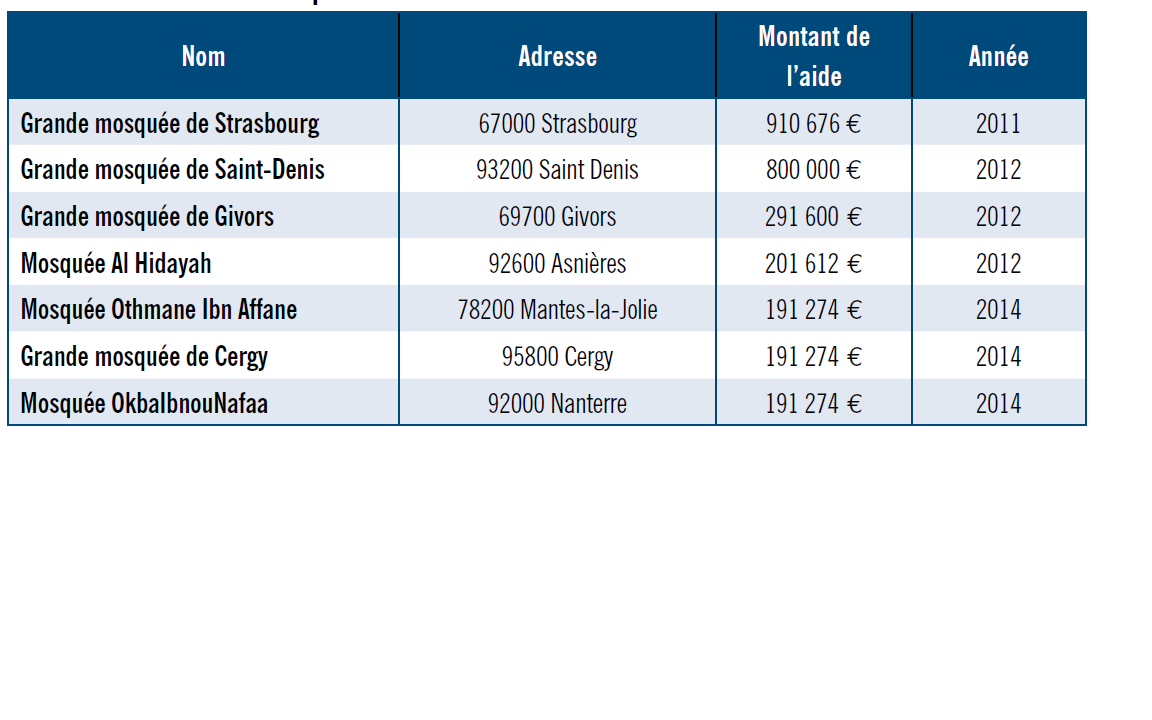
\includegraphics[width=\textwidth]{ImageIslamFrance/MosqueeArabieSaoudite.png}

    \label{fig:MosqueeArabieSaoudite}
\end{figure}

\paragraph{Le Qatar : la puissance financière et cathodique au service
d'une stratégie oblique}

Le Qatar opère davantage sur le paysage de l'islam français selon une
logique financière clientéliste et logistique que \emph{via} les
vecteurs traditionnels de l'islam consulaire. Et ce, en s'appuyant sur
des vecteurs médiatiques, déterritorialisés, tels que Tariq Ramadan,
ou « d'imams cathodiques » tels que le cheikh Youssef. Al-Qaradhâwî,
architecte de l'exportation télévisuelle de la vision islamiste qatarie,
qui \emph{via} l'émission « La charia et la vie » \emph{(al-sharî `a wa
al-hayât),} produite par la chaîne Al-Jazira, s'adresse directement aux
musulmans français maîtrisant l'arabe classique.

Selon Haoues Senigher, les mécènes qataris font \emph{« régulièrement
des dons à l'Union des Organisations Islamiques de France (UOIF),
héritière, et caisse de résonance française, de l'idéologie des Frères
musulmans que partage précisément une majorité d'officiels qataris. »}


%-----------------------------------------------------------------------------------
\section{L’émergence d’un courant réformiste}




%-----------------------------------------------------------------------------------
\section{Bibliographie de la partie}

BRUCE Benjamin, Governing islam abroad : the Turkish and Moroccan Muslim fields
in France and Germany, thèse de doctorat en sciences politiques, Sciences Po Paris,
sous la direction de Catherine Withol de Wenden, 2015,
https://www.theses.fr/2015IEPP0001 (une synthèse sera présenté par l’enseignant)
ZEGHAL Malika, « La constitution du Conseil Français du Culte Musulman :
reconnaissance politique d'un Islam français ? », Archives de sciences sociales des
religions [En ligne], 129 | janvier - mars 2005, mis en ligne le 09 janvier 2008, consulté
le 17 septembre 2020. URL : http://journals.openedition.org/assr/1113 ; DOI :
https://doi.org/10.4000/assr.1113
BAYLOCQ Cédric, « L’islam réformiste en France : des débats numériques à l’espace
socio-religieux », https://www.oasiscenter.eu/fr/islam-reformiste-en-france-debats-etprojets
Pour le lundi suivant : test de connaissance à mi-parcours (modalités à venir)


